\documentclass[border=4pt]{standalone}
\usepackage{fontspec}\setmainfont{Times New Roman}
\usepackage{tikz}\usetikzlibrary{arrows.meta,positioning,calc}
\begin{document}
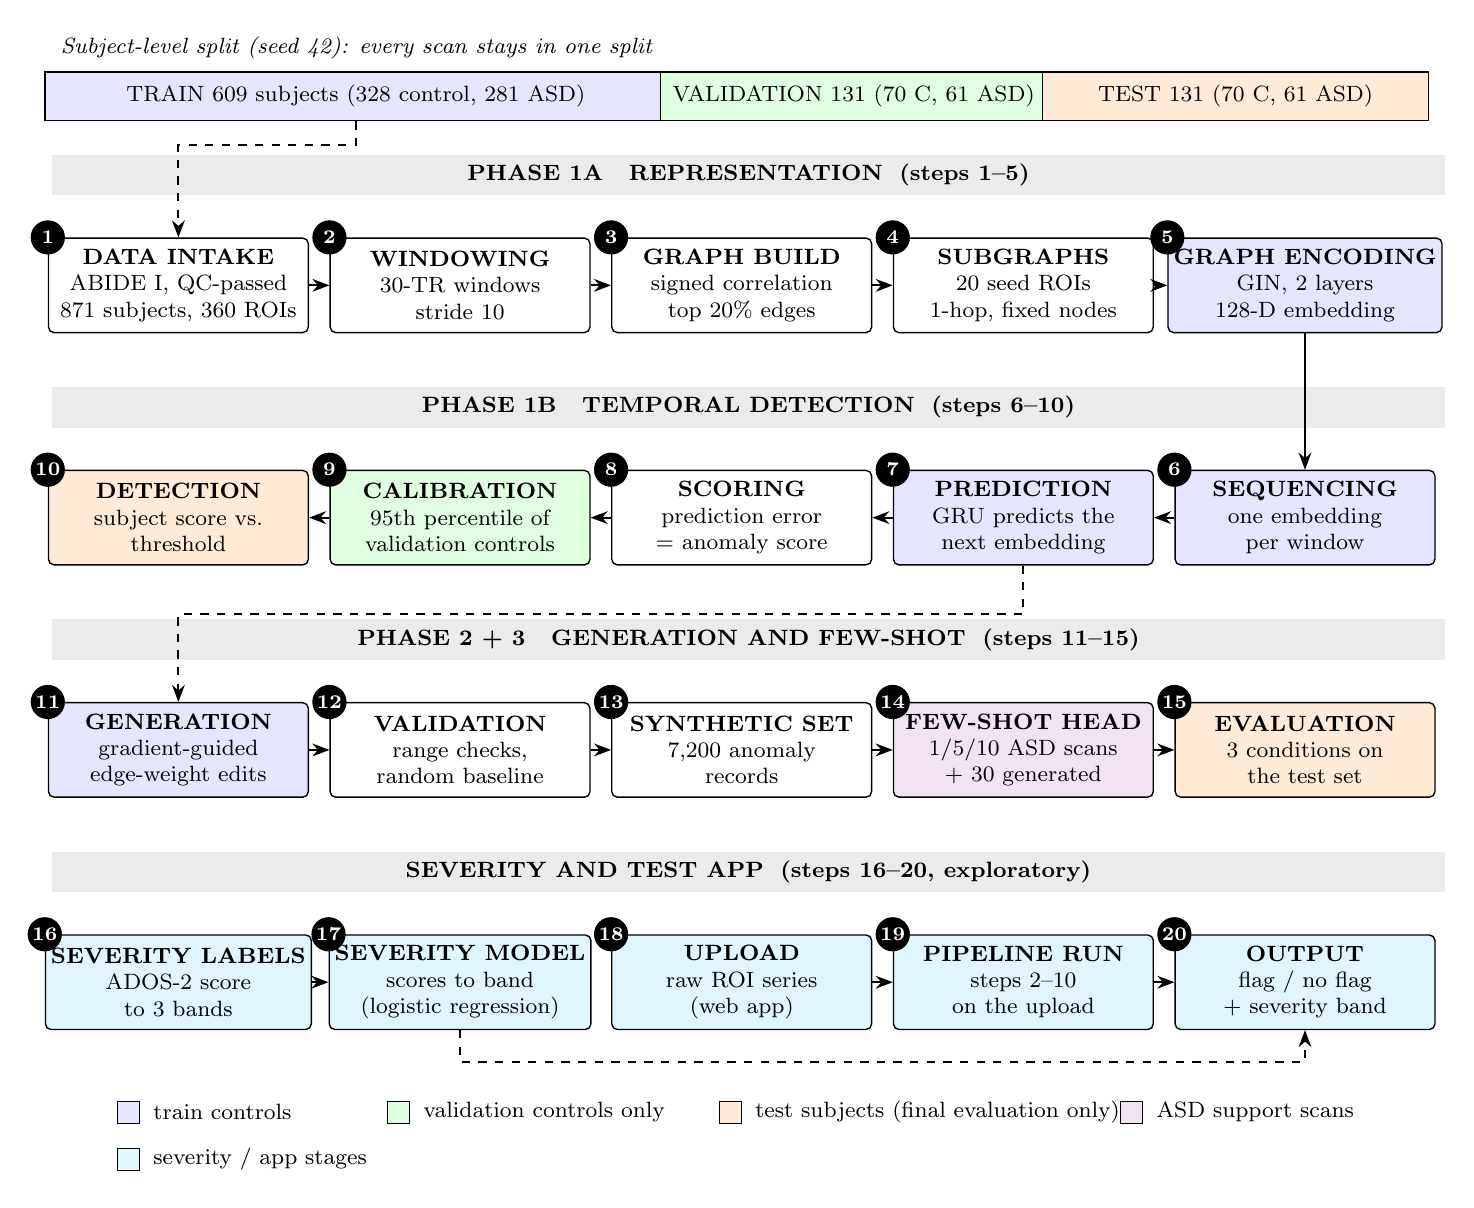
\begin{tikzpicture}[x=0.98cm,y=1cm,font=\footnotesize,>=Stealth,
 box/.style={draw,rounded corners=2pt,minimum width=3.3cm,minimum height=1.2cm,align=center,inner sep=2pt,line width=0.5pt,fill=white},
 trn/.style={box,fill=blue!10},val/.style={box,fill=green!12},tst/.style={box,fill=orange!16},sup/.style={box,fill=violet!11},sev/.style={box,fill=cyan!12},
 arr/.style={->,line width=0.7pt},
 band/.style={draw=none,fill=black!8,minimum height=0.5cm,minimum width=17.7cm,align=left,inner xsep=6pt,font=\footnotesize\bfseries},
 num/.style={circle,draw,fill=black,text=white,inner sep=0.6pt,minimum size=0.42cm,font=\scriptsize\bfseries}]
\node[draw,fill=blue!10,minimum width=7.9cm,minimum height=0.62cm,line width=0.5pt] (sp1) at (4.15,2.0) {TRAIN 609 subjects (328 control, 281 ASD)};
\node[draw,fill=green!12,minimum width=4.9cm,minimum height=0.62cm,line width=0.5pt] (sp2) at (10.6,2.0) {VALIDATION 131 (70 C, 61 ASD)};
\node[draw,fill=orange!16,minimum width=4.9cm,minimum height=0.62cm,line width=0.5pt] (sp3) at (15.55,2.0) {TEST 131 (70 C, 61 ASD)};
\node[font=\footnotesize\itshape,anchor=south west] at (0.2,2.35) {Subject-level split (seed 42): every scan stays in one split};
% ---- band 1
\node[band,anchor=west] at (0.2,1.0) {PHASE 1A \; REPRESENTATION \;(steps 1--5)};
\node[box] (b1) at (1.85,-0.4) {\textbf{DATA INTAKE}\\ABIDE I, QC-passed\\871 subjects, 360 ROIs};
\node[box] (b2) at (5.5,-0.4) {\textbf{WINDOWING}\\30-TR windows\\stride 10};
\node[box] (b3) at (9.15,-0.4) {\textbf{GRAPH BUILD}\\signed correlation\\top 20\% edges};
\node[box] (b4) at (12.8,-0.4) {\textbf{SUBGRAPHS}\\20 seed ROIs\\1-hop, fixed nodes};
\node[trn] (b5) at (16.45,-0.4) {\textbf{GRAPH ENCODING}\\GIN, 2 layers\\128-D embedding};
\foreach \a/\b in {b1/b2,b2/b3,b3/b4,b4/b5} \draw[arr] (\a.east)--(\b.west);
\draw[arr,dashed] (sp1.south)--++(0,-0.3) -| (b1.north);
% ---- band 2
\node[band,anchor=west] at (0.2,-1.95) {PHASE 1B \; TEMPORAL DETECTION \;(steps 6--10)};
\node[trn] (c1) at (16.45,-3.35) {\textbf{SEQUENCING}\\one embedding\\per window};
\node[trn] (c2) at (12.8,-3.35) {\textbf{PREDICTION}\\GRU predicts the\\next embedding};
\node[box] (c3) at (9.15,-3.35) {\textbf{SCORING}\\prediction error\\= anomaly score};
\node[val] (c4) at (5.5,-3.35) {\textbf{CALIBRATION}\\95th percentile of\\validation controls};
\node[tst] (c5) at (1.85,-3.35) {\textbf{DETECTION}\\subject score vs.\\threshold};
\draw[arr] (b5.south)--(c1.north);
\foreach \a/\b in {c1/c2,c2/c3,c3/c4,c4/c5} \draw[arr] (\a.west)--(\b.east);
% ---- band 3
\node[band,anchor=west] at (0.2,-4.9) {PHASE 2 + 3 \; GENERATION AND FEW-SHOT \;(steps 11--15)};
\node[trn] (d1) at (1.85,-6.3) {\textbf{GENERATION}\\gradient-guided\\edge-weight edits};
\node[box] (d2) at (5.5,-6.3) {\textbf{VALIDATION}\\range checks,\\random baseline};
\node[box] (d3) at (9.15,-6.3) {\textbf{SYNTHETIC SET}\\7,200 anomaly\\records};
\node[sup] (d4) at (12.8,-6.3) {\textbf{FEW-SHOT HEAD}\\1/5/10 ASD scans\\+ 30 generated};
\node[tst] (d5) at (16.45,-6.3) {\textbf{EVALUATION}\\3 conditions on\\the test set};
\foreach \a/\b in {d1/d2,d2/d3,d3/d4,d4/d5} \draw[arr] (\a.east)--(\b.west);
\draw[arr,dashed] (c2.south)--++(0,-0.62)-|(d1.north);
% ---- band 4
\node[band,anchor=west] at (0.2,-7.85) {SEVERITY AND TEST APP \;(steps 16--20, exploratory)};
\node[sev] (e1) at (1.85,-9.25) {\textbf{SEVERITY LABELS}\\ADOS-2 score\\to 3 bands};
\node[sev] (e2) at (5.5,-9.25) {\textbf{SEVERITY MODEL}\\scores to band\\(logistic regression)};
\node[sev] (e3) at (9.15,-9.25) {\textbf{UPLOAD}\\raw ROI series\\(web app)};
\node[sev] (e4) at (12.8,-9.25) {\textbf{PIPELINE RUN}\\steps 2--10\\on the upload};
\node[sev] (e5) at (16.45,-9.25) {\textbf{OUTPUT}\\flag / no flag\\+ severity band};
\foreach \a/\b in {e1/e2,e3/e4,e4/e5} \draw[arr] (\a.east)--(\b.west);
\draw[arr,dashed] (e2.south)--++(0,-0.4)-|(e5.south);
\foreach \i/\n in {b1/1,b2/2,b3/3,b4/4,b5/5,c1/6,c2/7,c3/8,c4/9,c5/10,d1/11,d2/12,d3/13,d4/14,d5/15,e1/16,e2/17,e3/18,e4/19,e5/20}
 \node[num] at (\i.north west) {\n};
% legend
\node[draw,fill=blue!10,minimum size=0.28cm,inner sep=0] at (1.2,-10.9) {}; \node[anchor=west] at (1.4,-10.9) {train controls};
\node[draw,fill=green!12,minimum size=0.28cm,inner sep=0] at (4.7,-10.9) {}; \node[anchor=west] at (4.9,-10.9) {validation controls only};
\node[draw,fill=orange!16,minimum size=0.28cm,inner sep=0] at (9.0,-10.9) {}; \node[anchor=west] at (9.2,-10.9) {test subjects (final evaluation only)};
\node[draw,fill=violet!11,minimum size=0.28cm,inner sep=0] at (14.2,-10.9) {}; \node[anchor=west] at (14.4,-10.9) {ASD support scans};
\node[draw,fill=cyan!12,minimum size=0.28cm,inner sep=0] at (1.2,-11.5) {}; \node[anchor=west] at (1.4,-11.5) {severity / app stages};
\end{tikzpicture}
\end{document}
